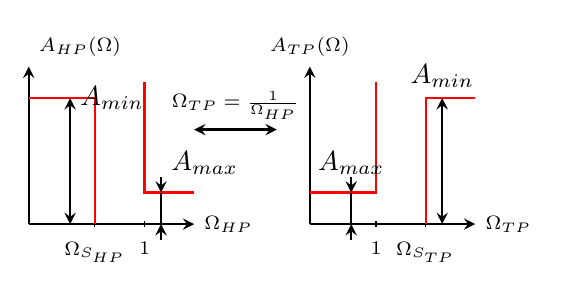
\begin{tikzpicture}[xscale=0.21, yscale=0.2]
% HP
\begin{scope}[local bounding box=HP]
	% Achsen zeichnen
	\draw[-{stealth},thick] (0,0) -- (10,0) node[right] {\scriptsize{$\Omega_{HP}$}};
	\draw[-{stealth},thick] (0,0) -- (0,10) node[above right] {\scriptsize{$A_{HP}(\Omega)$}};
	% Achsen beschriften
	\draw (4,-.2) -- (4,.2) node[below=4pt] {\scriptsize{$\Omega_{S_{HP}}$}};
	\draw (7,-.2) -- (7,.2) node[below=4pt] {\scriptsize{$1$}};
	% HP-Teil zeichnen:
	\draw[color=red, thick] (4,0) -- (4,8) -- (0,8);
	\draw[color=red, thick] (10,2) -- (7,2) -- (7,9); 
	\draw[{stealth}-{stealth}, thick] (2.5,0) -- (2.5,8) node[right] {$A_{min}$};
	\draw[-{stealth}, thick] (8,-1) -- (8,0);
	\draw[{stealth}-, thick] (8,2) -- node[above right] {$A_{max}$}(8,3);
	\draw[thick] (8,0) -- (8,2);
\end{scope}

% Verbindungspfeil
\draw[{stealth}-{stealth}, thick] (10,6) -- node[above] {\scriptsize{$\Omega_{TP} = \frac{1}{\Omega_{HP}}$}}(15,6);

% TP
\begin{scope}[local bounding box=TP]
% Achsen zeichnen
\draw[-{stealth},thick] (17,0) -- (27,0) node[right] {\scriptsize{$\Omega_{TP}$}};
\draw[-{stealth},thick] (17,0) -- (17,10) node[above] {\scriptsize{$A_{TP}(\Omega)$}};
% Achsen beschriften
\draw (21,-.2) -- (21,.2) node[below=4pt] {\scriptsize{$1$}};
\draw (24,-.2) -- (24,.2) node[below=4pt] {\scriptsize{$\Omega_{S_{TP}}$}};
% TP-Teil zeichnen:
\draw[color=red, thick] (24,0) -- (24,8) -- (27,8);
\draw[color=red, thick] (17,2) -- (21,2) -- (21,9); 
\draw[{stealth}-, thick] (19.5,2) -- node[above] {$A_{max}$}(19.5,3);
\draw[-{stealth}, thick] (19.5,-1) -- (19.5,0);
\draw[{stealth}-{stealth}, thick] (25,0) -- (25,8) node[above] {$A_{min}$};
\draw[thick] (19.5,0) -- (19.5,2);
\end{scope}
\end{tikzpicture}